\section{Modulære Fabrikker}

\begin{frame}{Modulære Fabrikker}{}
  
  \begin{itemize}
  \item<1-> Traditionel
    \begin{itemize}
    \item En opstilling bruges over en længere periode
    \item Ændrer produktion ved at omstille enkelte komponenter 
    \end{itemize}
  \item<2-> Modulær
    \begin{itemize}
    \item En opstilling bruges kortvarigt
    \item Ændrer også produktion ved at ændre fabriksopstillingen
    \end{itemize}
  \end{itemize}
\end{frame}

\subsection{Problem}

\begin{frame}{Problem}{}
\textit{How may we, given some order of items and set of avaliable modules, be able to
generate a factory configuration which has the fastest schedule of any other candidate
configuration?}
\end{frame}

\section{UPPAAL Model}
\begin{frame}{UPPAAL}{}
  \begin{itemize}
  \item<1->  Vælger at bruge til modelering da:
  \begin{itemize}
  \item Vi kan modelere tid
  \item Vi var allerede familære med UPPAAL og tidsautomater
  \end{itemize}
  \item<2-> Vores model
	\begin{itemize}
	\item  Fabrik og genstande opstilles som parallele processer, der kommunikerer indbyrdes.   
	\item Model Checker anvendes til at checke logiske egenskaber og generere \textit{shortest timed traces}.	
\end{itemize}	  
    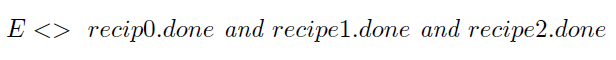
\includegraphics[width=0.9\textwidth]{figures/property.png}   
    
    \item<3-> Python interface til at instantiere konfigurationer
  \end{itemize}
\end{frame}

\subsection{Fra Virkelighed til Modeller}
\begin{frame}{Fra Virklighed til Modeller}{}
  \begin{itemize}
  \item<1->  Sammenligning med virkelig konfiguration:
  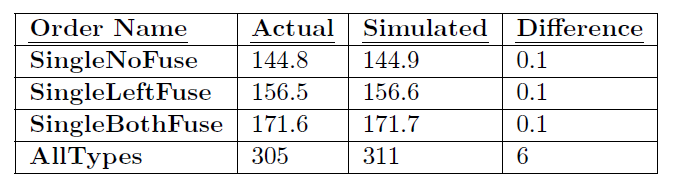
\includegraphics[width=0.8\textwidth]{figures/realTest.png}
  \item<2-> Afvigelse stiger i takt med at vores ordre bliver større.
\begin{itemize}
\item Måske på grund af at moduler hurtigere kan processere en mængde genstande  
\end{itemize}  
    \end{itemize}
\end{frame}

\subsection{Videreudvikling af Modellen}
\begin{frame}{Videreudvikling af Modellen}{}
    \begin{figure}
    \centering
    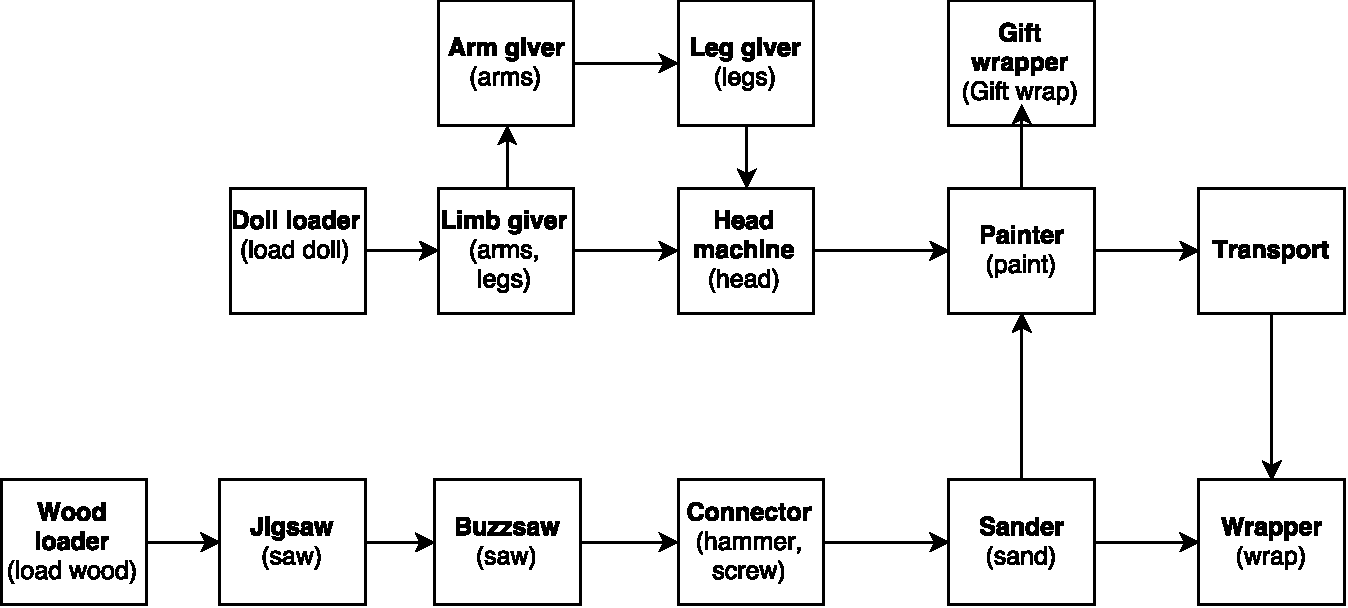
\includegraphics[width=1\textwidth]{figures/runningexample.pdf}
  \end{figure}
\end{frame}


\begin{frame}{Flere startpunkter}{}
  \begin{figure}
    \centering
    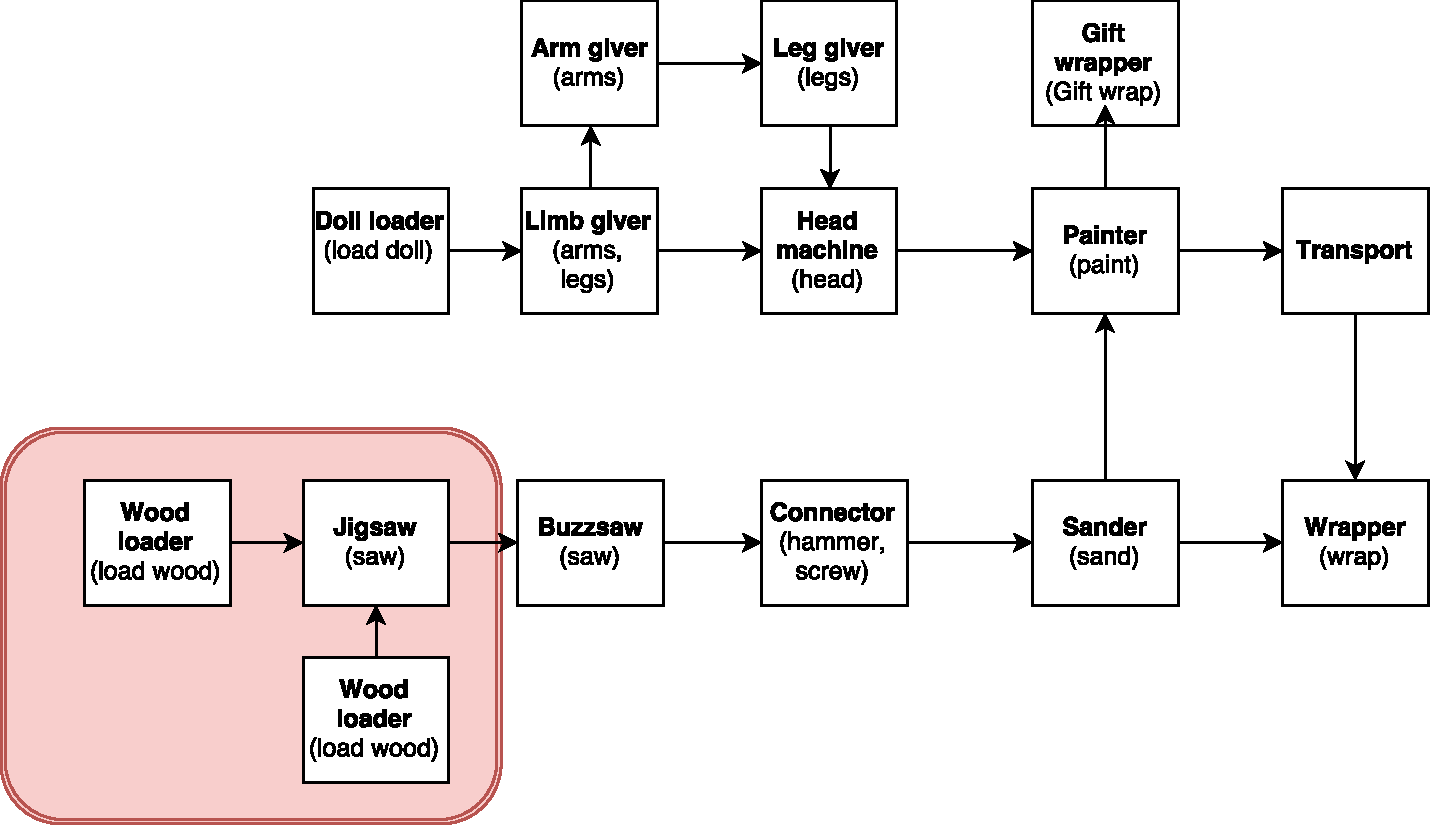
\includegraphics[width=1\textwidth]{figures/startAt2Modules.pdf}
  \end{figure}
\end{frame}


\begin{frame}{Parallel Seriel Eksekvering}{}
  \begin{figure}
    \centering
    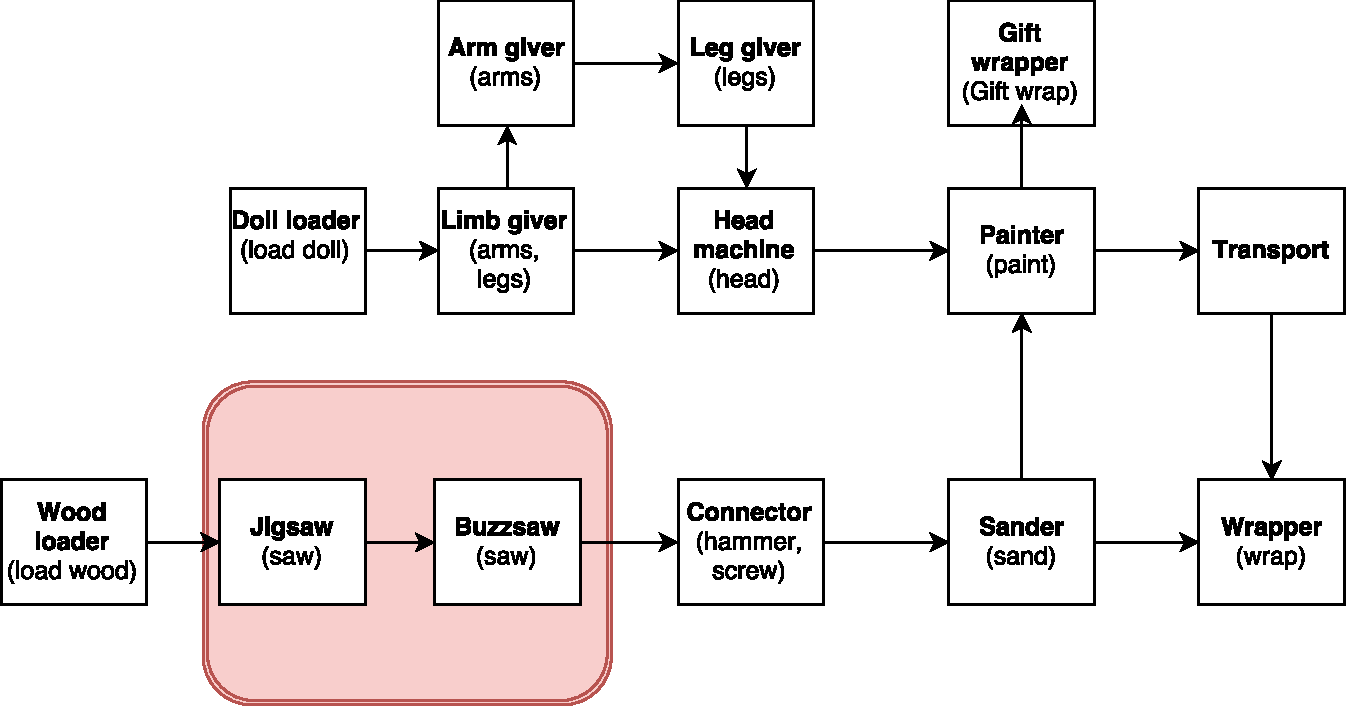
\includegraphics[width=1\textwidth]{figures/serialParallel.pdf}
  \end{figure}
\end{frame}

\begin{frame}{Kun en enkelt kø per modul}{}
  \begin{figure}
    \centering
    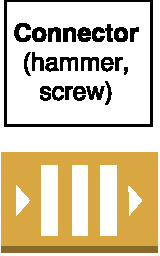
\includegraphics[width=0.3\textwidth]{figures/1queue.pdf}
  \end{figure}
\end{frame}

\begin{frame}{Kun en enkelt kø per modul}{En kø per retning}
  \begin{figure}
    \centering
    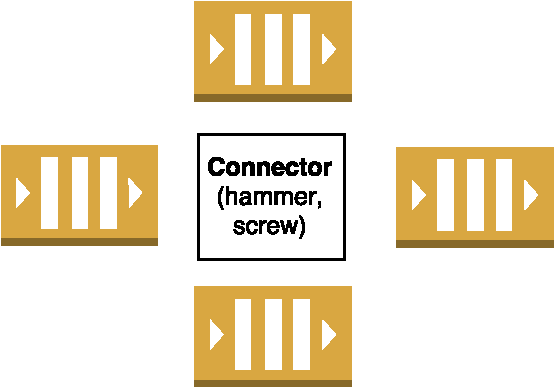
\includegraphics[width=0.7\textwidth]{figures/4Queues.pdf}
  \end{figure}
\end{frame}

\begin{frame}{Kun en enkelt kø per modul}{Intern kø}
  \begin{figure}
    \centering
    
\includegraphics[width=0.3\textwidth]{figures/internalQueue.pdf}
  \end{figure}
\end{frame}

\section{Transitionssystem}
\begin{frame}{Transitionssystem}{}
  \begin{itemize}
  \item<1-> Vi ønsker at søge igennem valide konfigurationer for at finde den bedste.
  \item<2-> Søgning tager udgangspunkt i en mængde af naive konfigurationer $C_{naive}$.
  \item<3->
  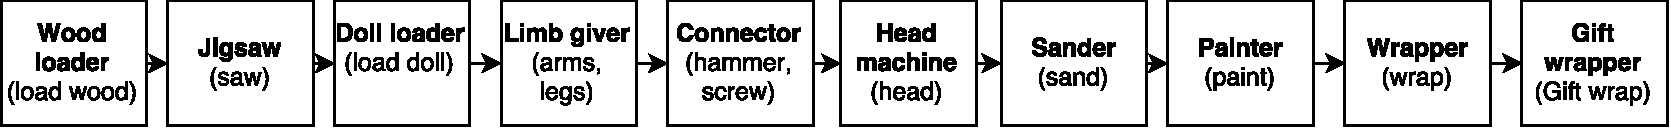
\includegraphics[width=0.9\textwidth]{figures/trivialexample.pdf}		    
    \end{itemize}
\end{frame}

\begin{frame}{Transitionssystem}{}
  \begin{itemize}
  \item<1-> Et transitionssystem defineres ved: $(C, \rightarrow)$
  \item<2-> C er mængden af alle konfigurationer
  \item<3-> $\rightarrow$ er transitionsrelationen mellem konfigurationer. 
  \item<4-> $(c_1,c_2) \in \rightarrow$, hvis dette kan udledes af en af vores regler og  $\exists c_{nx} \in C_{naive},  (c_{nx}, c_1) \in \rightarrow$
\end{itemize}    
\end{frame}
